\documentclass{beamer}

\usepackage[utf8]{inputenc}             %% Encoding
\usepackage{graphicx}

\usetheme{Goettingen}
\title{User Experience Engineering\\Design Thinking}
\author{Auer Thomas}
\date{\today}

\begin{document}
    \frame{\titlepage}

    \begin{frame}
        \tableofcontents
    \end{frame}
    
    \section{Idea gathering}
    \begin{frame}{Idea gathering}
        Lightning control in smart homes and similar environments
    \end{frame}

    \begin{frame}{Idea mindmap}
        \begin{figure}[H]
            \centering
            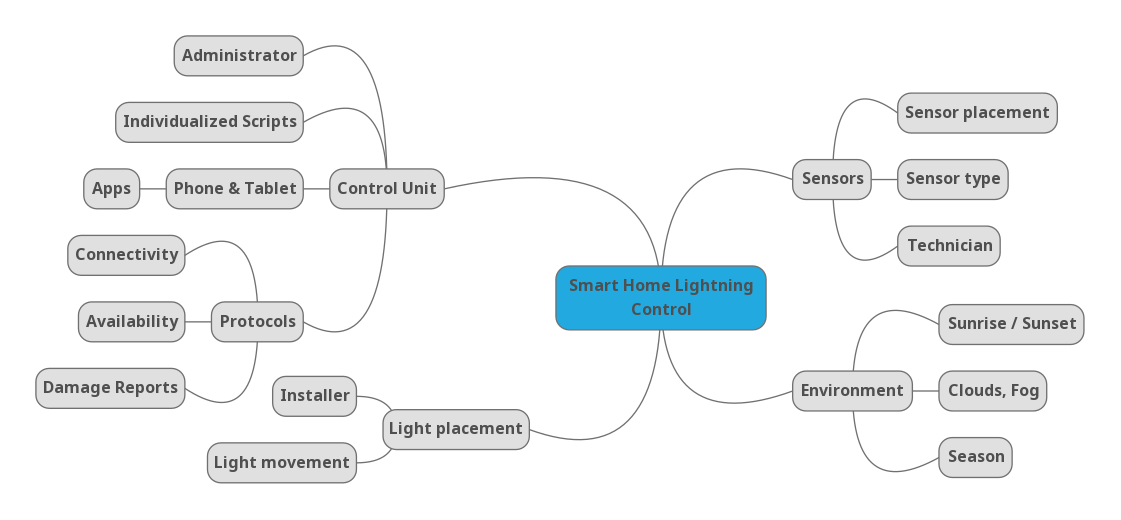
\includegraphics[width=1.0\textwidth]{Ideas.png}
            \label{fig:Ideas}
        \end{figure}
    \end{frame}
        

    \section{Doodle}
    \begin{frame}{Doodle - Control Unit}
        \begin{figure}[H]
            \centering
            
\includegraphics[width=2.25\textwidth]{Drawing_MOTH.png}
            \label{fig:Drawing_MOTH}
        \end{figure}
    \end{frame}

    \begin{frame}{Doodle - Environment}
        \begin{figure}[H]
            \centering
            
\includegraphics[width=2.25\textwidth]{Drawing_MOTH_Environment.png}
            \label{fig:Drawing_MOTH_Environment}
        \end{figure}
    \end{frame}

    \begin{frame}{Doodle - Lights}
        \begin{figure}[H]
            \centering
            
\includegraphics[width=2.25\textwidth]{Drawing_Lights.png}
            \label{fig:Drawing_Lights}
        \end{figure}
    \end{frame}

    \section{Choices}
    \begin{frame}{Choices}
        \begin{enumerate}
            \item MOTH interaction\\User feedback, system pulse
            \item MOTH programmability\\Data aggregation, remote API fetch, ...
            \item Sensor interaction\\Touch, Movement, Temperature, Sunshine, ...
            \item Sensor programmability\\What/How/When sensor activates and transmits
        \end{enumerate}
        -- Cannot interact with seasons or weather.
    \end{frame}

    \section{Storyboards}
    \begin{frame}{Storyboards}
        \begin{enumerate}
            \item MOTH individualization for user interaction
            \item MOTH programmability for advanced data aggregation
            \item Sensor interaction for different input/output methods
        \end{enumerate}
    \end{frame}


    \begin{frame}{MOTH individualization}
        \begin{figure}[H]
            \centering
            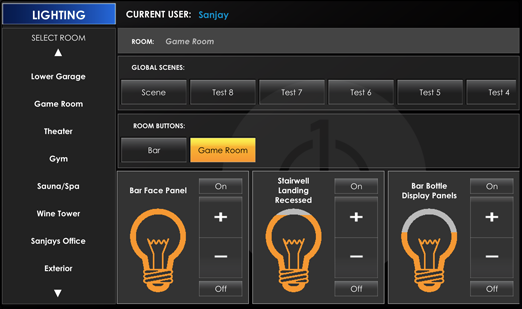
\includegraphics[width=1\textwidth]{Storyboard_UserInterface.png}
            \label{fig:Storyboard_UserInterface}
        \end{figure}
    \end{frame}

    \begin{frame}{MOTH programmability}
        \begin{figure}[H]
            \centering
            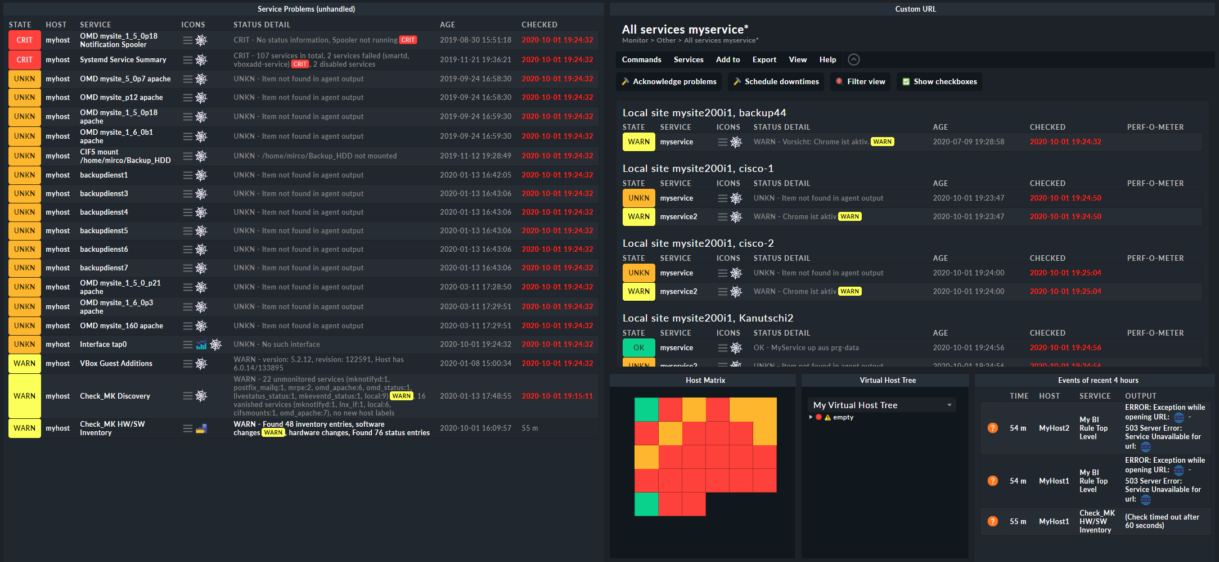
\includegraphics[width=1\textwidth]{Storyboard_Programmability.png}
            \label{fig:Storyboard_Programmability}
        \end{figure}
    \end{frame}

    \begin{frame}
        \begin{figure}[H]
            \centering
            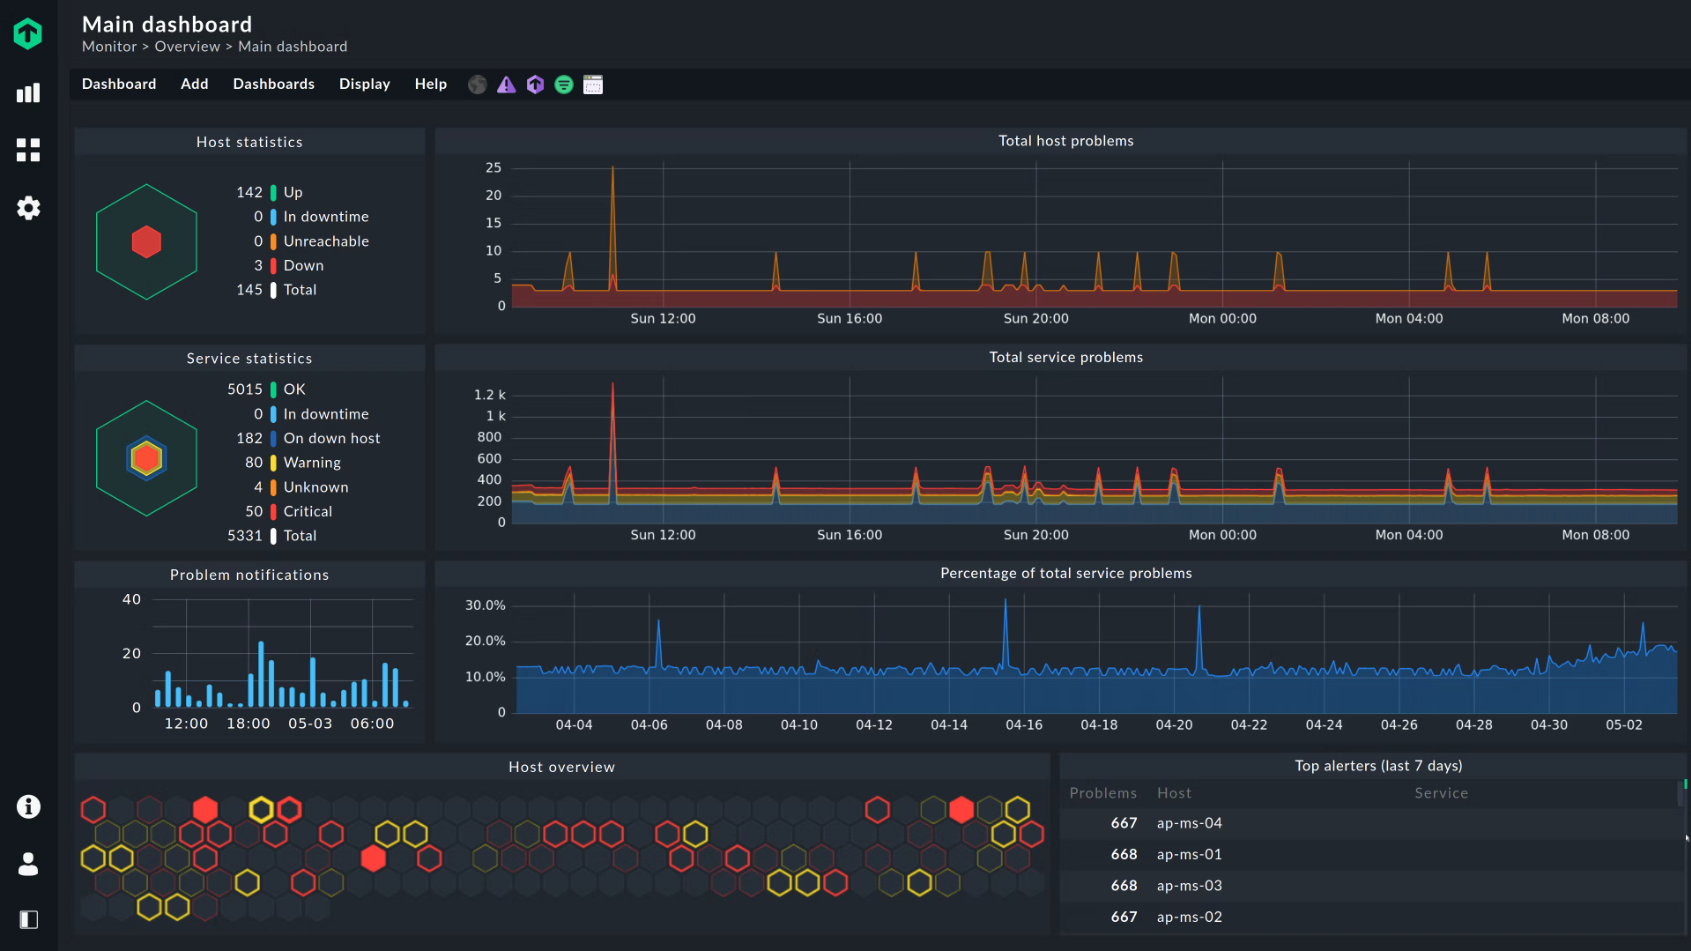
\includegraphics[width=1\textwidth]{Storyboard_UserFeedback.png}
            \label{fig:Storyboard_UserFeedback}
        \end{figure}
    \end{frame}

    \begin{frame}{Sensor interaction}
        \begin{figure}[H]
            \centering
            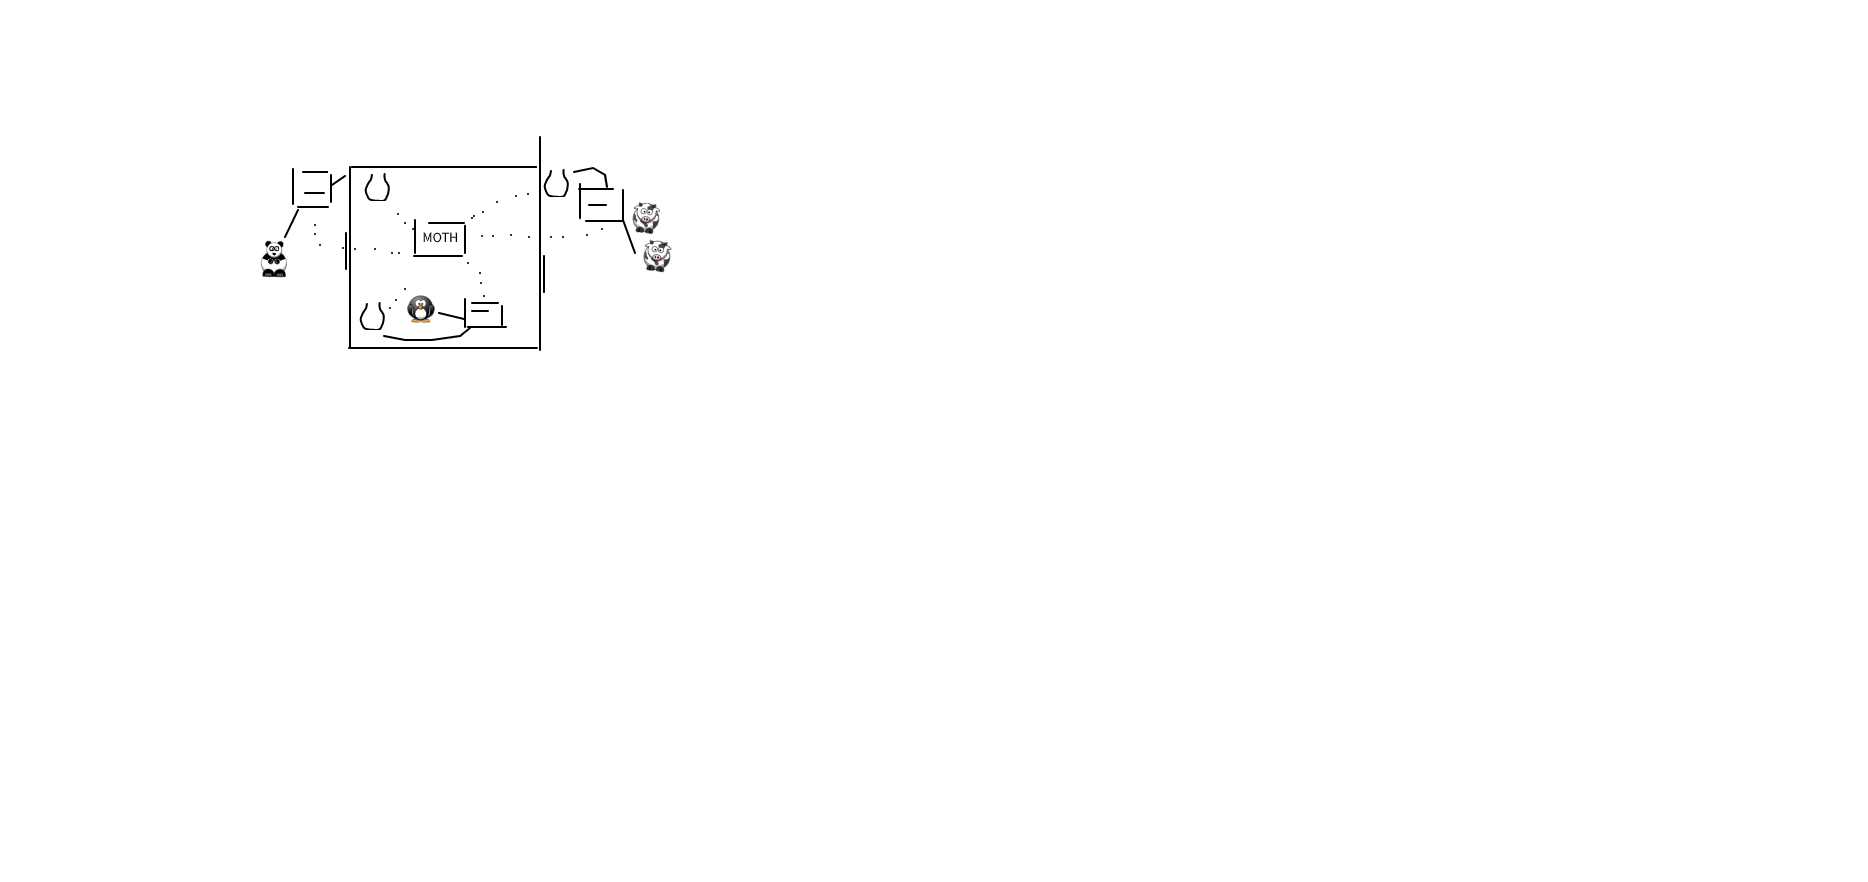
\includegraphics[width=2.7\textwidth]{Storyboard_Sensors.png}
            \label{fig:Storyboard_Sensors}
        \end{figure}
    \end{frame}





    \section{References}
    \begin{frame}{References}
        \begin{enumerate}
            \item Mindmap -- \url{https://app.mindmup.com/}
            \item Drawings -- \url{https://sketch.io/sketchpad/}
        \end{enumerate}
    \end{frame}


\end{document}